\documentclass[prb,preprint]{revtex4-1} 
% The line above defines the type of LaTeX document.
% Note that AJP uses the same style as Phys. Rev. B (prb).

\usepackage{amsmath}  % needed for \tfrac, \bmatrix, etc.
\usepackage{amsfonts} % needed for bold Greek, Fraktur, and blackboard bold
\usepackage{graphicx} % needed for figures
\usepackage{color}
\usepackage{ulem}
\usepackage{multirow}
\begin{document}

% Be sure to use the \title, \author, \affiliation, and \abstract macros
% to format your title page.  Don't use lower-level macros to  manually
% adjust the fonts and centering.

\title{Single-Photon Interference}


\author{Liza Mulder}
\email{emulder@smith.edu}
\affiliation{Department of Physics, Smith College, Northampton, MA 01063}


\author{Isabel Lipartito}
\email{iliparti@smith.edu}
\affiliation{Department of Physics, Smith College, Northampton, MA 01063}


\date{\today}



\begin{abstract}

It has been understood since the 19th century that light displays both wavelike and particle-like properties.  Light beams of differing phase interfere with each other and create observable light and dark fringes, as seen in Young's Double Slit experiment.  At the same time, light can be seen as a particle:  quanta of light, or photons, excite electrons to higher states of energy as seen in the photoelectric effect.  It is unlawful to attempt to classify light as a single entity.  We demonstrate the dual nature of light in the Single Photon Interference Experiment- a variation of Young's Double Slit Experiment.  We use a beam of light and a double slit apparatus with the confirmation that, within a certain probability, there is only a single photon in flight through the double slit device at any time.  Considering light to be a particle, we would expect to see two single bright fringes projected onto a screen.  However, even in the case of a single photon in flight at once, we still see dark and light interference fringes.  In this paper, we discuss the revolutionary implications of this result as well as how we might model these interference patterns.  We fit the Fresnel and Fraunhofer models of interference to our data and discuss the advantages and disadvantages of each.  We find that the Fraunhofer model is a better fit for our data, which makes sense as we were in the Fraunhofer regime, with a long box, long wavelength light source, and a thin slit.

\end{abstract}

\maketitle % title page is now complete


\section{Introduction} % Section titles are automatically converted to all-caps.
% Section numbering is automatic.

\textcolor{blue}{this is longer than it needs to be, and too repetitive!} \textcolor{blue}{you could delete everything in} \textcolor{red}{red} \textcolor{blue}{for example} \textcolor{red}{The revolutionary discovery of the dual wave-particle nature of light has been of significance beginning in the 19th century and continuing to today. } Isaac Newton \textcolor{red}{himself} believed defining light as a particle-like quantity (calling them corpuscles) would explain light refraction and reflection \cite{newton}.  \textcolor{red}{This idea was, however, superseded in the 19th century by the wave theory of light, due to the significant advances in electromagnetism.  The } interference experiments by Young in the early 19th century opposed the ideas of Newton and \textcolor{green}{demonstrated the wavelike nature of light}. \textcolor{blue}{given what you say elsewhere, this seems inconsistent to declare that the nature of light is wavelike. I think you mean to say that light has wavelike properties, or that it also behaves like a wave, under certain circumstances, or that it apparently demonstrated the wavelike nature of light...}   Young sent light beams through a single slit and observed diffraction of light waves passing through the slit.  \textcolor{blue}{misleading, since needs to be a single coherent beam of light that passes through both slits}\textcolor{green}{Young sent light beams through two slits and observed resultant interference patterns.}  In the latter part of the 19th century, discoveries by Maxwell, Faraday, and Hertz lead to the unification of the theories of electricity and magnetism.  Light was realized to be an electromagnetic wave- \textcolor{green}{a disturbance in an electromagnetic field.}\textcolor{blue}{I don't understand this, light IS a (traveling) electromagnetic field}  The contemporary theories of light bore little resemblance to the corpuscular theory of Newton.  \cite{david}

\textcolor{blue}{continue editing the next 2 paragraphs yourself, please!} 
However, support for the particle nature of light made a comeback in the early 20th century.  Perhaps the most famous example of this is Einstein's Nobel Prize winning explanation of the photoelectric effect, whose effects absolutely contradicted all predictions from the wave theory of light.  Einstein explained that quanta of light, to be called photons, strike the surface of a metal plate and excite electrons to freedom \cite{modern}.  The advent of quantum mechanics- a field based largely off the quantized nature of electromagnetic energy, further explored the particle-like properties of light.  A further example of this is Compton Scattering- a effect where a photon elastically collides with an electron and experiences a shift in wavelength.  

We know now that we can treat light as a particle: photons scatter and collide with matter.  We can also treat it as a wave: light beams constructively and deconstructively interfere with each other.  But can we call this an acceptable definition of light?  Can we say that we understand light?  The best way to test our understanding and perhaps \textcolor{green}{obfuscate} \textcolor{blue}{I think that word might mean the opposite of what you think it means!}  what we previously thought we understood is to undertake the Single Photon Interference Experiment.  We will take the same general set up as for the Young Double Slit Experiment:  beam of light, double slit, and means of viewing the output (see Methods section for a detailed description).  However, this time, we will reduce the intensity of light that we can be sure, to within a certain probability, that there is only a single photon in flight through the double slit apparatus at any time. \cite{teachspin}

\textcolor{blue}{This part in green probably belongs in the conclusion, since you haven't yet explained what the apparatus looks like and what these streaks might be}\textcolor{green}{ Even recalling the dual nature of light, we still want to insist that there should only be two bright streaks, parallel to the two slits.  We think, incorrectly, that each single photon must 'choose' a slit to pass through, and that is that!  There are no other photons going though the slits and we think that there should be no interference. } 

\textcolor{green}{The result of the single photon experiment is, to perhaps our surprise, an interference pattern, just like the one from Young's Experiment!  It seems like the photon 'went through two slits at once', or that it 'interfered with itself'.  The only lawful explanation we can provide at the moment is 'light is more complicated than we thought'. }

In this paper, we perform the Single Photon Experiment and examine the output double slit interference pattern produced by single photon interference.  We fit our output to two different models:  the Fraunhofer model and the Fresnel model, which draw upon different approaches to model the behavior of light.  The Fraunhofer model makes use of the picture of light as a plane wave reaching the two slits and propagating through it as a wave.  The Fresnel model considers the phase variation of an electromagnetic field with position in that field.  The Fresnel model is a sum over multiple paths from one location to another (here, from the source to the detector).  We discuss these models and our found fits in our analysis section.


\section{Methods}

We used the Teach-Spin\textcolor{red}{ "}2-Slit Interference One Photon at a Time" Apparatus for this experiment. \textcolor{red}{\texttt{in LaTeX we use `` not " to start a quote and '' not " to end one} The apparatus comes with a long black box containing an adjustable light source (with green filter to restrict wavelength and intensity), a 670nm laser source for alignment, four magnetic slit-holders along the length of the box for adding slits in the path of the light, and two detector options at the end: a photodiode (for laser light) and a photomultiplier tube (for lightbulb illumination). \textcolor{blue}{need figure 1 here, and it needs to show x, L, d, a  $\theta$ etc --- all the parameters used in the Fraunhofer model} on the figure}  We placed a single columnating slit in the first holder to focus the light from the lightbulb. This created vertical a single-slit diffraction pattern, which we centered on the next set of slits.  In the second slit holder, in the middle of the box, we placed the double-slit, and immediately following that we placed the slit blocker (a wide single-slit) so we could choose to allow light through one slit, both slits, or neither.  At the far end of the box we placed a single slit for the detector slit - by moving this slit holder lengthwise across the channel we could "scan" the interference pattern and measure photon counts at regular intervals.  

\textcolor{blue}{this paragraph needs to be edited for clarity and accuracy. For example, what do you mean by the PMT settings? why is it a voltage? why is it such a high voltage?  If it is a voltage, why do you refer to an electrical current? Is the current caused in some way by the voltage. The short pulse from the PMT output is a voltage spike of varying height. The Discriminator converts these spikes into a constant height rectangular pulse if the spikes exceed a threshold value, and no pulse if they don't.  Please re-read the handouts about how the PMT works, what the applied voltages and output voltages represent, what the discriminator actually does to shape the pulse, and how the threshold serves as a go - no-go criteria.}
Behind the detector slit was a photomultiplier tube (PMT).  The PMT generated an electrical current in response to the arrival of a photon, and adjusting the PMT settings changed the sensitivity - a low setting missed lower-energy photons, but a higher setting generated more noise.  We optimized this setting at 600V.  The short "pulse" from the PMT was translated into a voltage spike, which we sent to the pulse counter interval timer (PCIT).  The PCIT had a "discriminator" which screened out all pulses below a threshold voltage (in order to remove low energy noise, at the expense of some lower-energy photons) - we optimized this setting at 1.5V. The PCIT kept count of how many voltage "pulses" above its threshold voltage it received from the PMT within a 10s, 1s, or 0.1s time interval. More photon detections within the time interval indicated a high light intensity at that position of the detector slit, and photon detection levels near the background indicated a dark fringe in the pattern. By optimizing the apparatus alignment and the PMT and PCIT settings, we obtained a signal to noise ratio of roughly 2000 at the brightest point in the pattern.  \textcolor{red}{What does it mean to optimize the PMT and PCIT settings? How would someone actually do this, and how would they know what settings to choose? show us your signal + background / background  data or graph. Show us how you determined the best signal to noise setting!} 


Our green light bulb-power setting was at 5, which correlates to approximately $10^{3}$ photon events per second.  Green light photons have wavelengths near $.55 \mu $ meters, \textcolor{blue}{is the text in red providing useful information?}\textcolor{red}{frequencies near $5.5 \times 10^{14} $ Hz, and energies of around 2.3 eV.  The power level delivered by the photons is thus on the order of femtoWatts. }  The time in flight of the photons is on the order of nanoseconds (divide the meter of distance they travel by their speed, c).  Separation time between successive arrivals is on the order of milliseconds.  The PCIT will be devoid of photons about 99 percent of the time, \textcolor{green}{therefore.  This} is how we can say that there is a high probability of \textcolor{red}{single photon interference}\textcolor{blue}{have you defined this term? I think you are just trying to establish there is only one photon in the apparatus at a time, and later plan to indicate that means it somehow interferes with itself} , for the duration of our experiment.

To collect data, we moved the detector slit in increments of 0.1mm across the width of the interference pattern\textcolor{blue}{knowing the increment in mm is necessary, but it isn't that informative by itself. What does this translate to in terms of angle $\theta$?  or in terms of $x - x_0 / D$?}, measuring the photons counted for a 1s interval at each position.  The apparatus came with a micrometer which moved the detection slit holder 0.5mm every turn, and allowed us to read the slit's current position from the barrel.  In this way we could measure the photon counts at different positions.  We repeated this process with the slit blocker in different positions: once blocking the near slit and scanning the single-slit diffraction pattern generated by the far slit, once blocking the far slit and scanning the pattern produced by the near slit, once with both slits unblocked, and once with both slits blocked to get a read of the background.  We did three runs for each position of the slit blocker, to get a measure of the scatter in the results.  

Due to the random nature of the phenomena, and the method of data collection, we could not obtain an uncertainty for individual measurements we instead calculated error from the data for the three runs with the same settings. \textcolor{red}{Sorry, I don't understand this last statement. First, what do you mean by the same settings? Second, Earlier this semester,  you did a set of experiments demonstrating that photons obey Poisson statistics because they are randomly emitted, and therefore that the uncertainty was given by} $\sqrt{n}$ or more precisely, $\delta N_{photons} = \sqrt{N_{photons}}$, $\delta N_{background} = \sqrt{N_{background}}$ and $N_{counts} = N_{photons} + N_{backgrond}$\textcolor{red}{, etc etc? To determine $N_{\rm{photons}}$ and $\delta_{N_{photons}}$ you should have followed the same procedure, determining your background count, and then you subtracting that from the photons + background count, with an uncertainty for $N_{photons} = N_{counts} - N_{background}$ of $\delta_{N_{photons}} = \delta_{N_{counts}} + \delta_{N_{background}} $. Did you do this? If so, you need to say so, and give some indication what your S/N was for peaks and dips. THe error is not the same for each point, nor is the percent error. } 

  We analyzed this data and compared it to two theoretical models with Mathematica.  

\begin{figure}[h!]
\centering
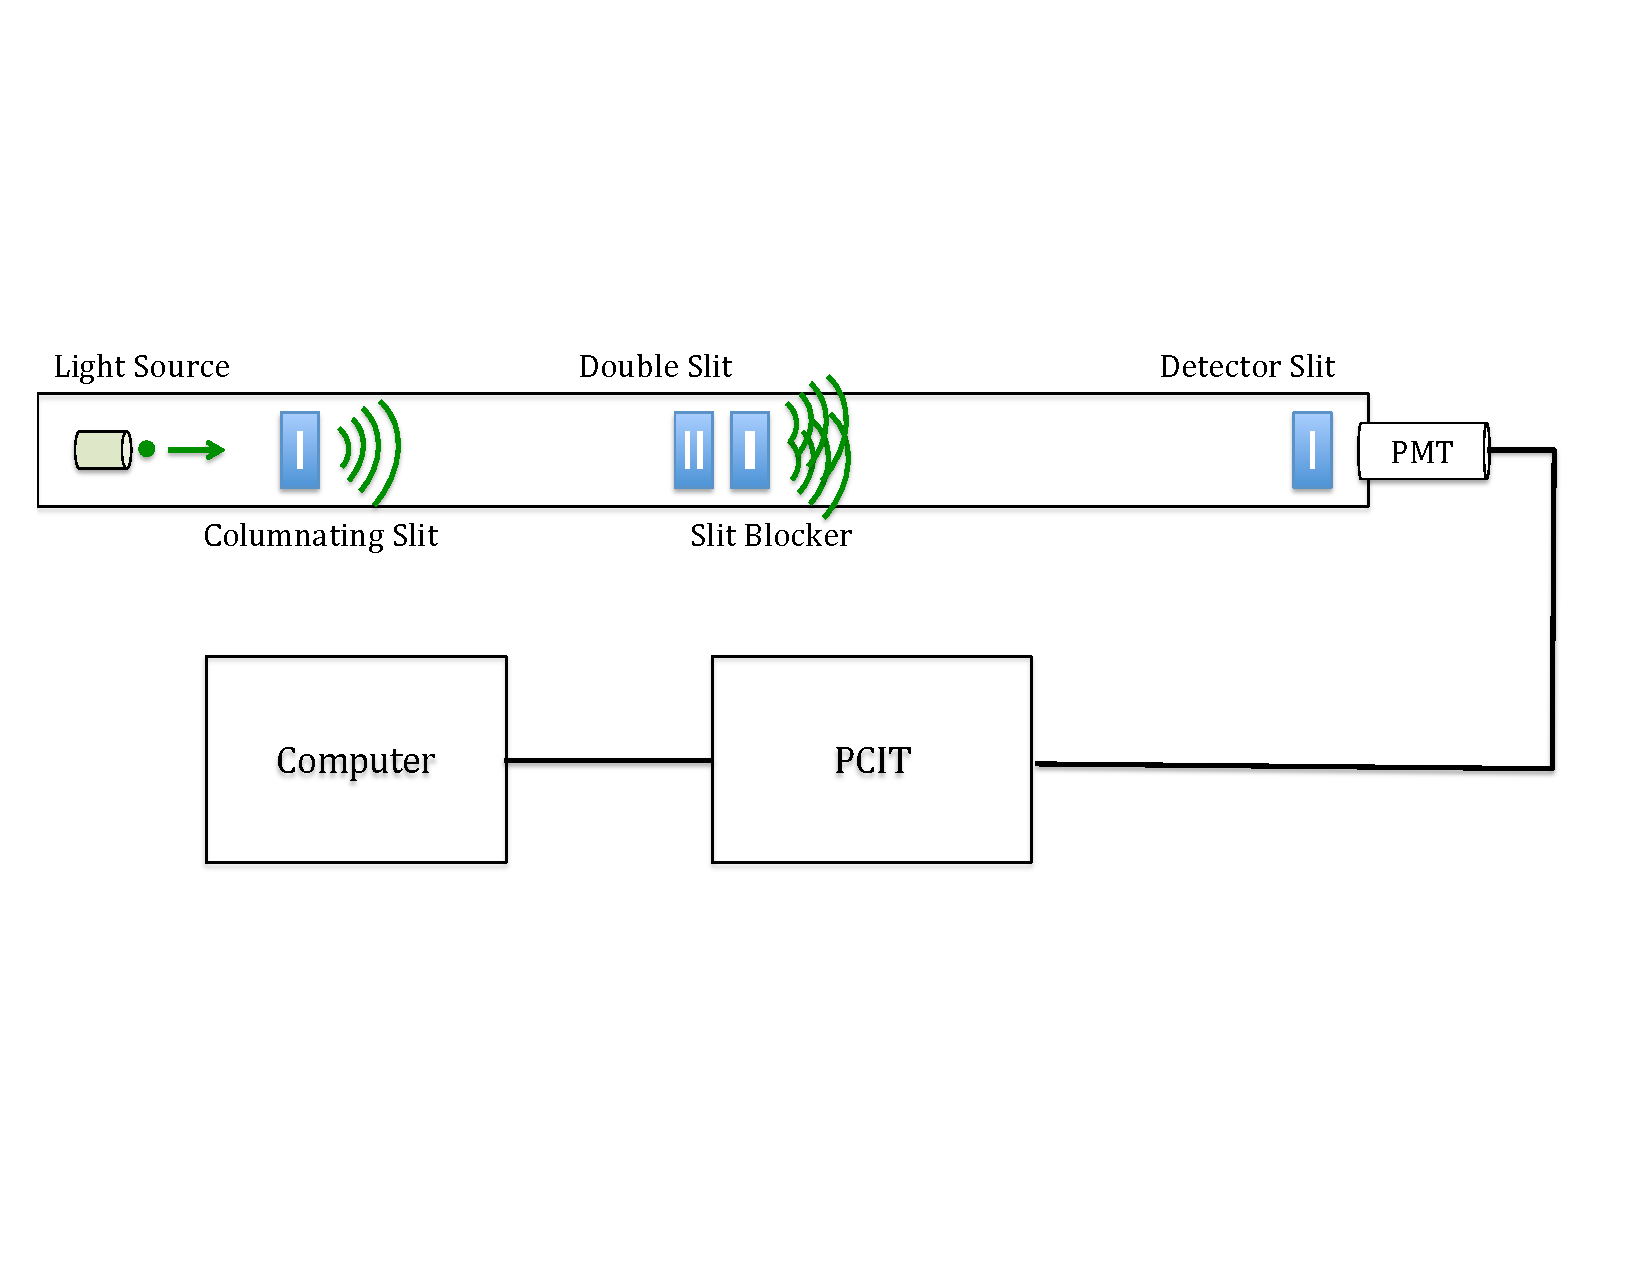
\includegraphics[width=6in]{set-up.pdf}
\caption{Teach-Spin apparatus to measure quantum interference: a 1m-long black box containing an adjustable light source (about 550nm), columnating single slit, double slit, slit blocker, detector slit, and photomultiplier tube (PMT) detector. We sent the PMT output to a pulse-counter interval timer (PCIT), and from there to the computer.\textcolor{blue}{add to this image some indication what $x$, $D$ and $\theta$ are, and if you can, add a sketch showing the funny-shaped pulse from the PMT is transformed to a digital rectangular pulse by the PCIT} }
\label{set-up}
\end{figure}

\section{Results}

The main result of our experiment was that we did indeed see single slit and double slit interference patterns, as we expected.  We then we fit two models to the data, to quantitatively verify our observation and agreement with theory.  Figures ~\ref{double_slit_plot} and ~\ref{single_slits_plot} show the detected light intensity (measured by the number of photon counts per second) at sequential micrometer settings (which give the position of the detector slit). The red data points are our raw data, showing the scatter across three runs, as well as the general trend. The larger, blue data points are the average values with error bars (the mean and standard deviation of the values from the three runs) for each value of position.  Our data has the form of single and double slit diffraction patterns, qualitatively.  In the analysis section we compare our data to two theoretical models. 

\begin{figure}[h!]
\centering
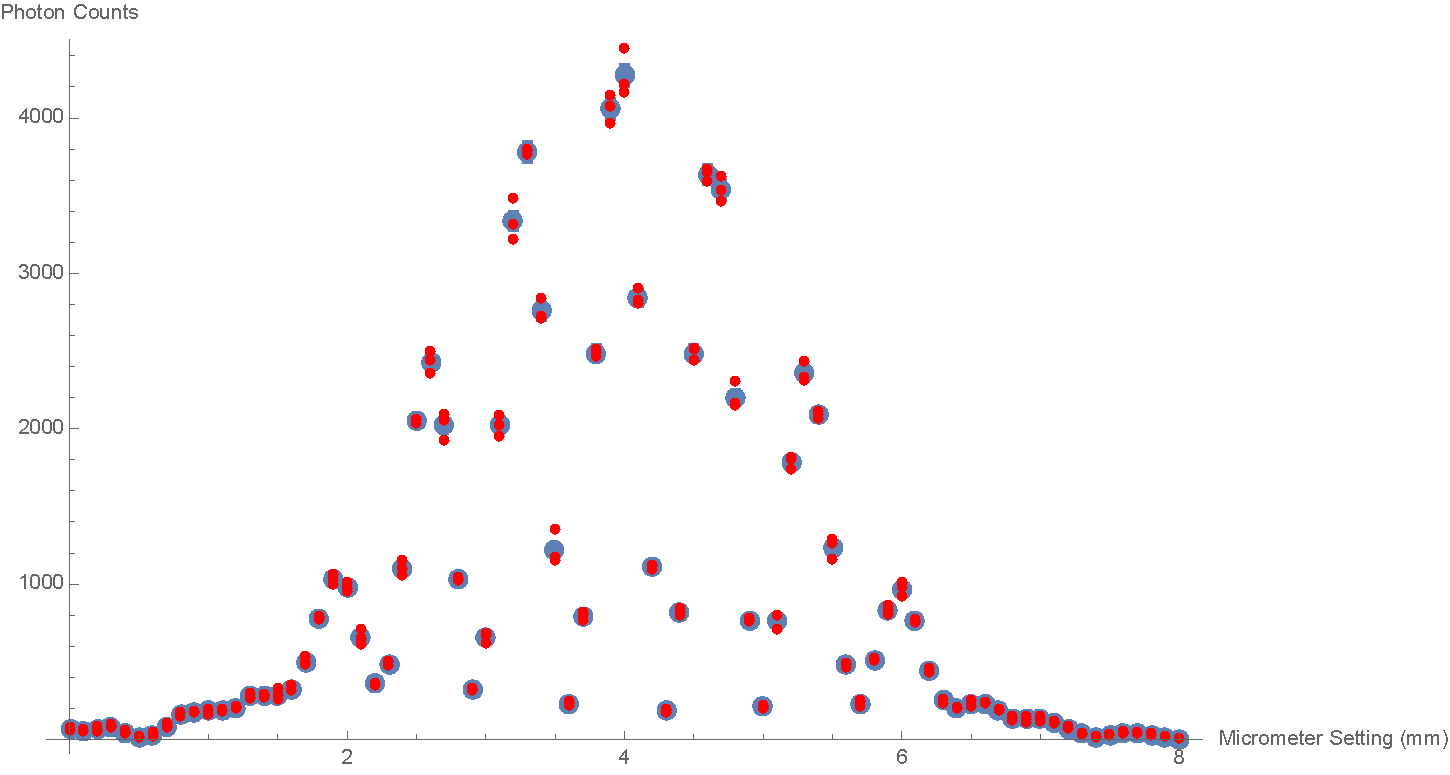
\includegraphics[width=6in]{double_slit_plot.pdf}
\caption{Our data for the double slit pattern.  Raw data is the small red points, averages with standard error are the larger blue points with error bars. }
\label{double_slit_plot}
\end{figure}

\begin{figure}[h!]
\centering
\begin{minipage}[b]{0.45\linewidth}
	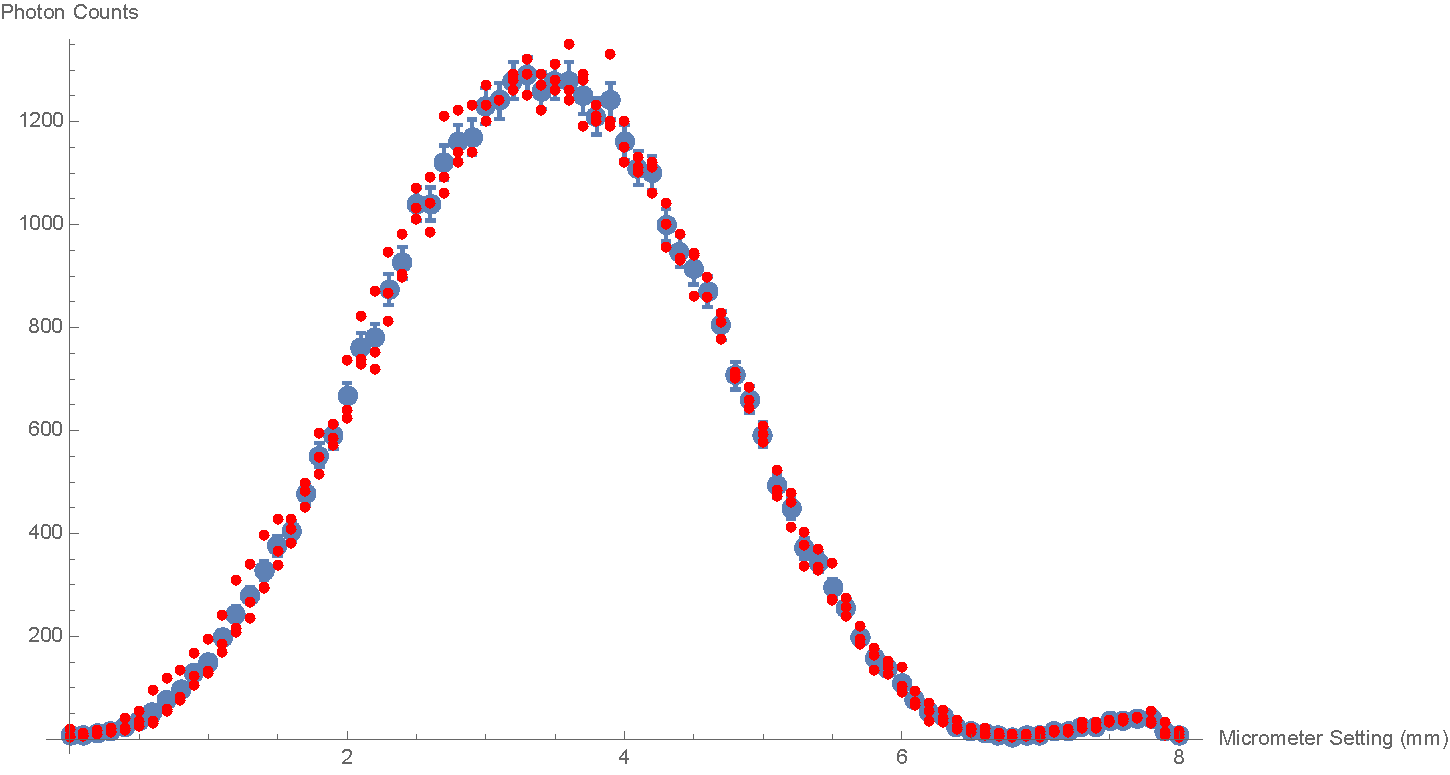
\includegraphics[width=3in]{far_slit_plot.pdf}
\end{minipage}
\quad
\begin{minipage}[b]{0.45\linewidth}
	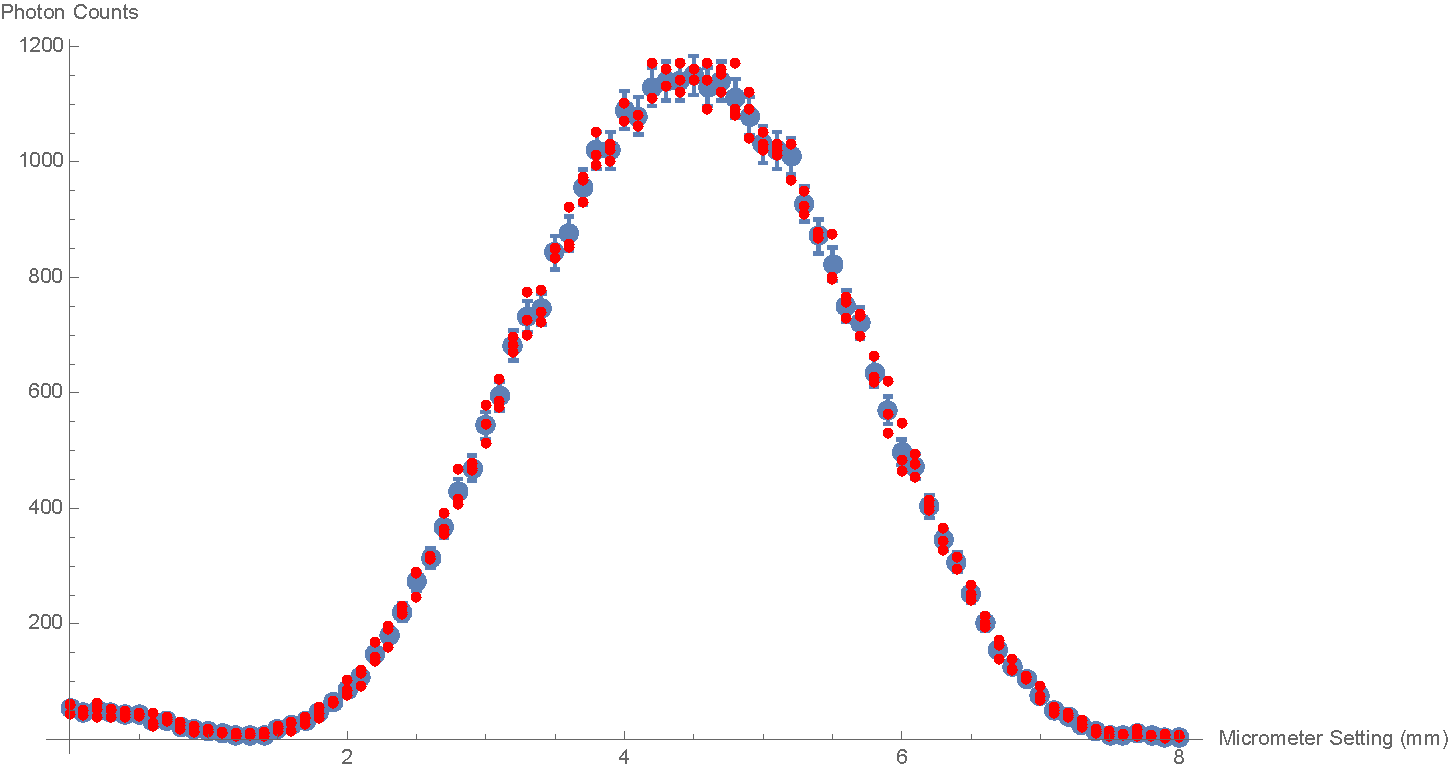
\includegraphics[width=3in]{near_slit_plot.pdf}
\end{minipage}
\caption{Our data for the single slit patterns. Raw data is the small red points, averages with standard error are the larger blue points with error bars. }
\label{single_slits_plot}
\end{figure}

\section{Analysis}

Below, we discuss the two models and our fits, as well as the goodness of these fits and their implications for this experiment and the theory of light.

We calculated fits for both the Fraunhofer Model and the Fresnel Model.  The two are applied in different regimes, determined by the Fresnel number: $F = \frac{a^2}{\lambda L}$.  $\lambda$ is the wavelength of the incident photons, a is the slit width, and l is the distance from diffracting slits to the detector slit.  When $F << 1$ the small slit is far from the detector screen, and the Fraunhofer model applies.  Nearer to the slit, where $F \approx 1$, the Fresnel model is more accurate. ~\cite{wolfram} The Fresnel number for our experiment is roughly $\frac{(0.1mm)^2}{555nm*500mm} \approx .036$.  Therefore the Fraunhofer model should be more appropriate, though neither is quite right - we would have to use a longer box, a longer wavelength light source, or thinner slits, to make the Fresnel number much smaller than $1$. 

\subsection{The Fraunhofer Model}

The Fraunhofer Model treats light as a wave and models it's arrival at a plane very far away. This is called "far field." It uses the assumption that the distance between the plane of the slit and the detector plane is much greater than the features of the slits or of the diffraction pattern.  This assumption allows the integral of complex exponentials which exactly describes the situation (shown later in the Fresnel model) to be approximated by the following sinusoidal equations, which are simpler. ~\cite{wolfram}

For the double slit case, the equation simplifies to:
\begin{equation}
I_{double}= I_{0}(\frac{\sin(\frac{\pi a}{\lambda}\sin(\frac{x-x_{0}}{D_{2}}))}{\frac{\pi a}{\lambda}\sin(\frac{x-x_{0}}{D_{2}})})^{2} \times \cos(\frac{\pi d}{\lambda}\sin(\frac{x-x_{0}}{D_{2}}))^{2}
\end{equation}

For the single slit cases, the equations are: 

\begin{equation}
I_{far}= \frac{I_{0}}{4}(\frac{\sin(\frac{\pi a}{\lambda}\sin(\frac{x-x_{1}}{D_{2}}))}{\frac{\pi a}{\lambda}\sin(\frac{x-x_{1}}{D_{2}})})^{2} 
\end{equation}

\begin{equation}
I_{near}= \frac{I_{0}}{4}(\frac{\sin(\frac{\pi a}{\lambda}\sin(\frac{x-x_{2}}{D_{2}}))}{\frac{\pi a}{\lambda}\sin(\frac{x-x_{2}}{D_{2}})})^{2} 
\end{equation}

Where $I_0$ is the \textcolor{red}{amplitude} of the central maximum {\textcolor{red}{the use of amplitude is misleading here, since $I$ and $I_0$ etc are actually intensities, not  wave amplitudes}, $a$ is the width of the slits, $x_0$ is the location of the central maximum in the double-slit pattern, $x_1$ is the location of the central max in the far single-slit pattern, $x_2$ is the location of the central max in the near single-slit pattern, $D_2$ is the distance between the slit and the detector, $\lambda$ is the wavelength of the light, $x$ is the position of the detector slit, and $c$ is a vertical offset. \textcolor{blue}{don't forget to explain what $d$ is in the double slit experiment, and to also show these variables on a figure}. 

\textcolor{red}{$d$ is the slit separation from slit center to slit center. As drawn, your }$d$ \textcolor{red}{is too short by} 2 x $a/2$. \textcolor{red}{You will need to offset the} $a$ \textcolor{red}{symbol and double-headed arrow that indicates the slit width in FIgure 6}

We fit our data to the Fraunhofer model by plotting our entire data set against the model, using the manufacturer's values for the slit widths, slit separation, and light wavelength, and our observed maximum intensity and central maximum locations.  We then modified these values to try and get a better fit of the function to the data, estimating a satisfactory fit by eye.  As the manufacturer did not give error for most of their parameters, we had to guess at the limits within which we could vary the parameter values. \textcolor{red}{it would help to list those original values --- in addition to your adjusted values --- in your Table I} However, we obtained a good fit for the double slit pattern (with the exception of the very edges), and decent fits for the single slit patterns.  Our single slit data was slightly off because we had not centered the columnated light exactly on the two slits, so one slit had approximately $10\%$ more illumination than the other.  As the fit assumed equal illumination from both slits, the amplitudes did not match.  

\begin{figure}[h!]
\centering
\begin{minipage}[b]{0.45\linewidth}
	\includegraphics[width=3in]{far_slit_Fraunhofer_plot.pdf}
\end{minipage}
\quad
\begin{minipage}[b]{0.45\linewidth}
	\includegraphics[width=3in]{near_slit_Fraunhofer_plot.pdf}
\end{minipage}
\caption{Our data for the single slit patterns with the Fraunhofer formula on top. The parameters we used are in Table ~\ref{parameters}. Raw data is the small red points, averages with standard error are the larger blue points with error bars. }
\label{single_slits_Fraunhofer_plot}
\end{figure}

\begin{figure}[h!]
\centering
\includegraphics[width=6in]{double_slit_Fraunhofer_plot.pdf}
\caption{Our data for the double slit pattern with Fraunhofer fit on top.  Raw data is the small red points, averages with standard error are the larger blue points with error bars. }
\label{double_slit_Fraunhofer_plot}
\end{figure}

\begin{table}[h!]
\centering
\caption{Parameter values for our fits. We started with the values given in the apparatus manual ($a, d, \lambda$), measured ($D_1, D_2$), or estimated from the plots ($I_0, x_0, x_1, x_2, c$).  We then optimized (within the uncertainty for each parameter) to get the Fraunhofer fits as close to the data as possible. }
\begin{ruledtabular}
\begin{tabular}{lc}
Parameter & Fit value       \\
Counts/sec at central max $I_0$     & 4400 counts/sec \\
Slit width $a$       & 0.085 mm        \\
Slit separation $d$       & 0.406 mm        \\
Light wavelength $\lambda$ & 555 nm          \\
Location of central max (double slit) $x_0$     & 3.95 mm         \\
Location of central max (far slit) $x_1$     & 3.45 mm \\
Location of central max (near slit) $x_2$ & 4.45 mm \\
Offset $c$       & 3.6 counts/sec. \\
Distance from columnating slit to diffracting slits $D_1$     & 338 mm          \\
Distance from diffracting slits to detector slit $D_2$     & 500 mm         
\end{tabular}
\end{ruledtabular}
\label{parameters}
\end{table}

\subsection{The Fresnel Model}

The Fresnel model does not use the approximation from the Fraunhofer model, \textcolor{green}{since the detector plane is assumed to be in the}\textcolor{red}{ "}\textcolor{green}{near field,}\textcolor{red}{"}\textcolor{green}{ closer to the slits}. 

\textcolor{blue}{The statement in green above is not quite right, and this is an important point for later. More accurate would be to say that the Fresnel model doesn't assume that we are in the ``far field'' limit, and is most commonly used in the ``near field'' limit since the Fraunhofer model doesn't apply there. As long as you use enough terms in the taylor series expansion for the path lengths (see page 8-4 of the TeachSpin manual, for example) it can be accurate everywhere, and should be an even better description. it is often referred to as a `near-field'' solution b/c it works in that limit even when the Fraunhofer model doesn't!} 

Therefore the equation is left in it's complex exponential form, and the distances between the slits and between slit and detector become very important.  ~\cite{wolfram} This equation is very difficult to solve, but a computing program such as Mathematica can run the calculation.  \textcolor{blue}{That is an impressive and non-obvious calculation, so you should include that program as an appendix.} 

\textcolor{red}{In the equations below, what is the point of the 42.044 term, and what does it mean? Why not factor it into} $I_0$? [\textcolor{red}{also, You seem to be saying that the I terms in the sum over paths approach below (and in the Section 8 part B of the TeachSpin manual) are intensities, but they aren't. In this case, they are amplitudes, which is why you need to find the absolute square to find the intensity.} 

The single slit cases:

\begin{equation}
I_{near}=I_{0}*42.044*|e^{\frac{2 \pi i D_{1}}{\lambda}}*e^{\frac{2 \pi i D_{2}}{\lambda}}*\int_{x_{0}-\frac{d}{2}}^{x_{0}+\frac{d}{2}+a} \! e^{\frac{2 \pi i (x_{0}-y)^{2}}{D_{1} \lambda}}*e^{\frac{2 \pi i (y-z)^{2}}{D_{2} \lambda}} \, \mathrm{d}y |^{2}
\end{equation}





\begin{equation}
I_{far}=I_{0}*42.044*|e^{\frac{2 \pi i D_{1}}{\lambda}}*e^{\frac{2 \pi i D_{2}}{\lambda}}*\int_{x_{0}+\frac{d}{2}}-a^{x_{0}-\frac{d}{2}} \! e^{\frac{2 \pi i (x_{0}-y)^{2}}{D_{1} \lambda}}*e^{\frac{2 \pi i (y-z)^{2}}{D_{2} \lambda}} \, \mathrm{d}y |^{2}
\end{equation}

\textcolor{red}{The limits appear to be written wrong on these equations, and there is certainly a formatting error in the 2nd equation.  I might be misunderstanding what you mean by near and far here, but for example,  shouldn't the first equation read: }

\begin{equation*}
I_{near}(z)=I_{0}*42.044*|e^{\frac{2 \pi i D_{1}}{\lambda}}*e^{\frac{2 \pi i D_{2}}{\lambda}}*\int_{y = \left(x_{0}-\frac{d}{2}\right) - \frac{a}{2}}^{\left(x_{0}-\frac{d}{2}\right) + \frac{a}{2}} \! e^{\frac{2 \pi i (x_{0}-y)^{2}}{D_{1} \lambda}}*e^{\frac{2 \pi i (y-z)^{2}}{D_{2} \lambda}} \, \mathrm{d}y |^{2}
\end{equation*}


\begin{equation*}
I_{near}=I_{0}*42.044*|e^{\frac{2 \pi i D_{1}}{\lambda}}*e^{\frac{2 \pi i D_{2}}{\lambda}}*\int_{\left(x_{0}+\frac{d}{2}\right) - \frac{a}{2}}^{\left(x_{0}+\frac{d}{2}\right) + \frac{a}{2}} \! e^{\frac{2 \pi i (x_{0}-y)^{2}}{D_{1} \lambda}}*e^{\frac{2 \pi i (y-z)^{2}}{D_{2} \lambda}} \, \mathrm{d}y |^{2}
\end{equation*}

The double slit case is simply the sum of the waveforms generated by each slit: 
\begin{equation}
I_{double}=I_{near}+I_{far}
\end{equation}

\textcolor{blue}{true if you recognize these are amplitudes and that you are adding amplitudes rather than intensities here. But then you need to find} $ {I^*}_{\text{double}} * I_{\text{double}}$ \textcolor{blue}{to find the measured light intensity.} 

The parameters have the same meanings as in the Fraunhofer model, with the addition of $D_1$, the distance from the columnating slit to the diffracting slit, and with the exception of $x$, $y$, and $z$: $x$ is the location of the columnating slit, $y$ is the location of the diffracting slit, and $z$ is the location of the detector slit.  Figure ~\ref{Fresnel_diagram} shows the parameters and their use in the Fresnel model.  

\begin{figure}[h!]
\centering
\includegraphics[width=4in]{Fresnel_diagram.png}
\caption{The set-up and variables used in the Fresnel Approximation. Note that the variable "Z" in the Fresnel formula is what we've been calling "X" in our other calculations - the position of the detector slit.\textcolor{red}{$d$ is the slit separation from slit center to slit center. As drawn, your }$d$ \textcolor{red}{is too short by} 2 x $a/2$. \textcolor{red}{You will probably need to offset the} $a$ \textcolor{red}{symbol and double-headed arrow that indicates the slit width in FIgure 6 to show d properly}}
\label{Fresnel_diagram}
\end{figure}

\begin{figure}[h!]
\centering
\includegraphics[width=6in]{double_slit_Fresnel_plot.pdf}
\caption{Our data for the double slit pattern with Fresnel fit on top.  Raw data is the small red points, averages with standard error are the larger blue points with error bars. \textcolor{blue}{It looks like there might be an error in the numerical values used in this calculation, because you have 9 peaks in your fit but only 7 peaks in your data. That is, the ratio }$d/{\lambda}$ \textcolor{blue}{appears to be 9/7 too large.}}
\label{double_slit_Fresnel_plot}
\end{figure}

\begin{figure}[h!]
\centering
\begin{minipage}[b]{0.45\linewidth}
	\includegraphics[width=3in]{far_slit_Fresnel_plot.pdf}
\end{minipage}
\quad
\begin{minipage}[b]{0.45\linewidth}
	\includegraphics[width=3in]{near_slit_Fresnel_plot.pdf}
\end{minipage}
\caption{Our data for the single slit patterns with the Fresnel formula on top. The parameters we used are in Table ~\ref{parameters}. Raw data is the small red points, averages with standard error are the larger blue points with error bars. }
\label{single_slits_Fresnel_plot}
\end{figure} 

After fitting our data, we computed the reduced chi-square value for each fit (see Table ~\ref{chi-square}).  All few of the values were very large.  By examining the distance of individual points from the fit, however, we realized that the majority actually had small deviations from the line, with a few outliers which weighted the fit.  Even so, from the graphs it is clear that no single set of parameter values allows all the fits to match the data.  We optimized our parameters for the Fraunhofer double-slit fit - as these parameter values were within the uncertainty of what we knew they should be, we kept these parameters.  However, the other fits each had some sort of systematic offset from the line.  

\begin{table}[h!]
\centering
\caption{Reduced chi-square values for our fits. }
\begin{ruledtabular}
\begin{tabular}{cccc}
                            &             & 0mm \textless x\textless 80mm & 20mm \textless x \textless 60mm \\
\multirow{3}{*}{Fraunhofer} & Double Slit &57.67                      & 9.76                         \\
                            & Far Slit    & 3.31                       & 1.16                        \\
                            & Near Slit   & 0.326                       &        0.091           \\
\multirow{3}{*}{Fresnel}    & Double Slit &          155.41               & 86.70                         \\
                            & Far Slit    & 4.80                       & 0.311                         \\
                            & Near Slit   & 4.23                       &1.01                       
\end{tabular}
\end{ruledtabular}
\label{chi-square}
\end{table}


\section{Discussion}

Our biggest question with this experiment was why, while we obtained clear data of the interference patterns, these results deviated from the theoretical models, sometimes by a great amount.  In particular the Fresnel model could not be made to fit our data very well, even with the best estimations of our parameters, but considering that we were far from the regime of the Fresnel model, we did not find this to be too strange. \textcolor{red}{I think you should first consider a simpler possible explanation for the discrepancy: It looks like there is an error in the numerical value of }$d/{\lambda}$ \textcolor{red}{used in this calculation, because you have 9 peaks in your fit but only 7 peaks in your data. The value used appears to be 9/7 too large. ANother possibility is that you mistakenly added \textit{a}  = 0.085 to \textit{d},  using \textit{d} = 0.491 instead of 0.406 (or made an equivalent error in the specification of the integral limits).  Please check that you used the same value for \textit{d}, \textit{a} and }$\lambda$ \textcolor{red}{in your Fresnel fit that you used in your Fraunhofer fit, and that you defined the ranges of the integrals properly for the Fresnel fit. }

In addition, we observed that the Fresnel model fit very well at the very edges of our pattern:  it was able to follow the subtle bumps and wiggles of that region.  The Fresnel model also replicated the "wavy offset" of our minima, while the Fraunhofer model had each minima come down to zero.  This offset was several times too large to be attributed to our background noise, so it is likely due to some characteristics of the Fresnel model which the Fraunhofer model approximated away.  The Fraunhofer model did better in the middle- around the more defined light and dark fringes.  The Fresnel model does not fit the inner light and dark fringes at all.  It fits the most central bright fringe, and then is offset from the rest of the bright fringes (the fit peaks are too narrow, and so there are more in the same space).  We are not exactly sure why this is so, but we have a few speculations.    The Fraunhofer model is designed to take advantage of the wave nature of light, and is not equipped to handle any 'edge effects' resulting due to the finite nature of the detector slit.  The Fresnel model, on the other hand, is a sum over all paths from the source to the detector, and is more equipped to take into account imperfect paths and imperfections around the edges of the pattern.   However, we were far off from the Fresnel regime and close to the Fraunhofer regime, so that might explain how the Fraunhofer model fit very well our central interference pattern and Fresnel did not - overall, our graphs and reduced chi-square values agree better with the Fraunhofer model than with the Fresnel model.  \cite{teachspin}

In order to gauge better the fits of the models to the experimental data, we would want to repeat this experiment using smaller incremental turns of the micrometer.  There are large gaps in our plotted fits that could be closed with tighter measurements.  We possibly would want to turn the micrometer by .05 mm instead of .1 mm increments.  We would also want to more precisely measure ourselves the parameters that went into our Fraunhofer and Fresnel fits:  slit width (a), slit separation (d), and the distances from the different slits to the detector slit ($D_{1} and D_{2}$), rather than relying on the uncertain reported values from the Two-Slit Interference, One Photon at a Time manual.  We could also gauge some error estimates for these values and propagate them, in our fits, so our fits would themselves have an error range.

An interesting project would be to continue this experiment and made adjustments to bring the set-up closer to the Fraunhofer and Fresnel limits.  For Fraunhofer, we would want to repeat this experiment with thinner slit widths, larger wavelength photons, and a longer box.  For Fresnel, we would want to repeat this experiment with larger slits, shorter wavelength photons, and a shorter box.  Taking into account practicality (maybe a 50 meter box is not going to be possible!), we could adjust the Fresnel number in both cases to ensure we are in the correct regime for our data to resemble the Fraunhofer or Fresnel model.  It would be exciting to confirm the Fraunhofer and/or Fresnel model, and probe the limits of these models further.

Regarding the quantum mechanical theory of this experiment, we did indeed observe single photon interference.  If a single photon was moving through a two-slit apparatus at any one time, how did the interference happen?  It seems like the photon somehow 'knew' about the two slits and managed to self-interfere (a bit of an obfuscating idea!).  It is certainly unfair to continue to think of the photon as a classical particle or classical wave propagating through space.  Perhaps it is better to think of a sort of quantum amplitude propagating through space- an amplitude whose absolute square would give information on where and when one is likely to observe the photon interaction event.  The picture by which we observe the photon events are the double slit interference patterns which depict favored and not-so-favored photon detection spots (according to the propagating quantum amplitude) as light and dark interference fringes, respectfully.  \cite{teachspin}

The double slit experiment may be rather old, but it is certainly still relevant today.  Contemporary physicists are exploring the wave-particle duality of other particles aside from photons.  In 1999, the double slit experiment was successfully performed with buckyballs and it has been relatively recently been performed with electrons.   \cite{bucky}.  The application of quantum mechanics to explain the behavior of subatomic particles and their interactions via fields, known as quantum field theory (QFT), is a new and relevant division of physics.  Contemporary research in Quantum Electrodynamics, the QFT to explain the interaction of light and matter, involves introducing a wave function for the photon and mathematically modeling interactions between matter and light \cite{iwo}.  Quantum field theory might help us probe the nature of the photon and better understand its seemingly 'impossible' doings.

\section{Conclusion}

We successfully performed the single photon interference experiment and observed the expected single-slit diffraction patterns and double-slit interference patterns predicted by theory.  We fit our resulting data to the Fresnel and Fraunhofer models and found that the Fraunhofer model was a better fit for our data (it generated far lower reduced chi-square values).  This makes sense as we were in the Fraunhofer regime (thin slit width and long box).  We explored the quantum mechanical implications of single photon interference and discussed quantum electrodynamics, a theory developed to apply quantum mechanics to the electromagnetic field and better physically and mathematically understand the mysterious nature of the photon.

\begin{thebibliography}{3}
 \bibitem{newton}Use of Hamilton's Canonical Equations to Rectify Newton's Corpuscular Theory of Light:  A Missed Opportunity.  Buenker et al, 2004.  Sov. J. Chem. Phys. 22 (2003) 124
 \bibitem{david}Introduction to Electrodynamics, 4th Edition.  David J. Griffiths, 2012.  Addison Wesley.
\bibitem{wolfram}Weisstein, Eric W. Wolfram Science World, "Fraunhofer Diffraction," "Fresnel Diffraction," "Fresnel Number." 2007. 
\bibitem{teachspin} TeachSpin Instruction Manuals.  Two-Slit Interference, One Photon at a Time (TWS1-B).  TWS1B-PCIT1 Instruction Manual. Rev. 1.0 6/2013
\bibitem{modern} Six Ideas That Shaped Physics: Unit Q - Particles Behaves Like Waves.  Thomas Moore.  McGraw-Hill Science/Engineering/Math; 2 edition, 2003.
\bibitem{bucky} Wave-Particle Duality of C60 Molecules.  Arndt et al, 1999.  Nature Vol. 401
\bibitem{iwo}The Photon Wave Function.  Iwo Bialynicki-Birula, 1996.  Coherence and Quantum Optics VII, Eds. J. H. Eberly, L. Mandel, and E. Wolf
Plenum, New York 1996, p. 313
\end{thebibliography}
\end{document}
